\title{Pylon: On-chain composable security middleware v0.1 (draft)}

\author{
        Anton Zagorodnikov (antzagos@gmail.com) \\
        Anton Mozgovoy (a@mozgovoy.me) \\
}
\date{}

\documentclass[12pt]{article}

\usepackage{pdfpages}

\usepackage{xcolor}

\usepackage{graphicx}
\usepackage{bytefield}
\usepackage{makecell}
\usepackage{auto-pst-pdf}
\usepackage{amsmath}

\usepackage{url}

\usepackage[ruled,vlined]{algorithm2e}

\usepackage{hanging}

\usepackage{tikz}
\newcommand*\circled[1]{\tikz[baseline=(char.base)]{
            \node[shape=circle,draw,inner sep=2pt] (char) {#1};}}

\usepackage[]{hyperref}
\hypersetup{
    pdftitle={Holyheld: Treasury implementation v0.1 (draft)},
    pdfauthor={antzagos@gmail.com},
    pdfsubject={solidity},
    pdfkeywords={blockchain, ethereum, solidity, smart contracts},
    bookmarksnumbered=true,
    bookmarksopen=true,
    bookmarksopenlevel=1,
    colorlinks=true,
    pdfstartview=Fit,
    pdfpagemode=UseOutlines,
    pdfpagelayout=TwoPageRight
}

\begin{document}
\maketitle

\textbf{\footnotesize Legal Disclaimer}\scriptsize
~~Nothing in this article is an offer to sell or the solicitation of an offer to buy any tokens. Mover is publishing this article solely to receive feedback and comments from the public.

Nothing in this article should be treated or read as a guarantee or promise of how Mover’s business or the tokens will develop, or the utility of the tokens and smart contract functions. This article outlines current plans, which could change at its discretion. And the success of which will depend on many factors outside Mover’s control, including but not limited to market-based conditions and factors within the data and cryptocurrency industries. Any statements about future events are based solely on Mover’s analysis of the issues described in this article. That analysis may prove to be incorrect.

\begin{abstract}
This article describes the concepts and implementation details of a Mover Pylon: a smart contract that serves as a security middleware layer. It provides means to implement access separation, integration with security roles defined in other smart contracts, and means to provide safe execution of various smart contract calls by trusted third parties. Pylons are designed to introduce minimal gas overhead for transaction execution and concise structure to stay manageable and transparent.
\end{abstract}

\newpage

%1. Introduction
%2. Key concepts
%	1. Responsibility division;
%	2. Key distribution;
%	3. Gas overhead (more admin expenses, but cheap execution);
%	4. Identity (address) protection;
%	5. Time-related and action-related constraints;
%	6. Permission quantification;
%	7. Two-actor case and shutdown;
%	8. Actor power and vetoing;
%	9. Executor management;
%	10. Emergency committee;
%3. Use cases (Situations modeling)
%	1. n of m multi-actor pylon;
%	2. Pylon governed by a DAO;
%	3. Hierarchical placement;
%	4. Risks and attack vectors;
%	5. Mover infrastructure scenario;
%4. Implementation considerations;
%	1. Main interfaces description;
%	2. View functions;
%	3. Creation options;



\section{Introduction}\normalsize

When actors are making transactions on a blockchain (hereafter, we would imply the Ethereum mainnet), the critical component of such interaction is the process of signing a transaction with the EOA (externally-owned address) private key. This process is verified by a blockchain node before the transaction gets into the memory pool, is broadcasted, and eventually gets included in the block, changing the blockchain state.

The private key safety is crucially important. It is a single item that proves ownership of a particular address. Needless to say that the security of the private key depends solely on the key owner. Here are some of the security aspects for a better understanding:
\begin{itemize}
\item{A private key is not a password and cannot be changed;}
\item{A private key cannot be blocked or frozen by a certain party (e.g., a network operator blocking a SIM card or a bank freezing a credit card);}
\item{A private key is too long and complicated to remember by humans reliably (at least, most of them) and, accordingly, to type in manually when required;}
\item{Modern software (wallets) are generating private keys from a seed phrase (mnemonic), which began as an HD (hierarchically-deterministic) approach proposed in \href{https://github.com/OpenBitcoinPrivacyProject/bips/blob/master/bip-0047.mediawiki}{BIP47}\cite{bip47} (submitted by Justus Ranvier in 2015). The seed phrase is easier to remember but potentially can expose several private keys. Therefore, the seed phrase is commonly not stored in wallets. Instead, private keys are stored in encrypted form, secured via a separately provided password, which the user is entering when the private key access is required. If the user loses access to the wallet software and loses seed phrase, access is irrecoverably lost;}
\item{ Some advanced users prefer to sign transactions via a separate (e.g., network-disconnected) device or specialized hardware (cold storage wallet software).}
\end{itemize}

These considerations underline the importance of the private key safety and dire consequences if exposed or lost. Ethereum does not provide (and is out of the base network scope) means of managing private key security, so there are possible situations that have no means of graceful resolving:
\begin{itemize}
\item{If a user loses access to a wallet software, private key, seed phrase, etc., then such user activity on-chain would be stalled, and effectively such EOA ceases to operate;}
\item{If a malicious third party gets access to a private key, then such EOA can't be restricted for making any actions. There are no additional checks to verify created transaction;}
\end{itemize}

\medskip
If we look at this from a smart contract management perspective, this involves additional risks and attack vectors:
\begin{enumerate}
\item{Some of the EOAs could be automated services acting off-chain. Such addresses execute transactions to manage the smart contracts' actions, thus, having the private key in their possession. If a part of the infrastructure is compromised, that could lead to exposure of such private keys;}
\item{Human actors that have EOAs with elevated permissions in the smart contracts can lose access to their EOAs or expose them to third-parties (equipment loss, theft, damage, etc.);}
\item{Smart contracts are becoming more complicated and distributed. Managing them becomes more error-prone. In case of an error or a private key exposure it is hard (or impossible) to provided fixes in a graceful manner;}
\end{enumerate}

\medskip
However, there are emerging means and practices to mitigate some of the risks and difficulties:
\begin{enumerate}
\item{Multisignature wallets. \emph{Pros:} divided responsibility, ability to change the signers, convenient UI; \emph{Cons:} gas-expensive, tailored to regular spending transactions (not smart-contract interaction), inflexibility for temporal quantitative restrictions (more on that in the next paragraphs);}
\item{\href{https://docs.openzeppelin.com/contracts/2.x/access-control}{Role-based permissions}\cite{permissions_roles} in the smart contracts. Such permissions require careful maintenance and role-management (DEFAULT\_ADMIN\_ROLE essentially gives all roles access through providing role management);}
\item{Contracts upgradeability. This method invokes a tremendous improvement for maintainability: expanding features, correcting errors without a full redeployment of a contract, and migration (which, if possible, is complicated and often expensive). However, the address that has permission to upgrade a smart contract has tremendous power and significantly reduces trust in a deployed smart contract;}
\item{Timelock mechanisms for elevated actions. Sometimes a quick action is required (e.g., if there’s a critical bug that needs to be fixed as soon as possible). Monitoring timelock functions is not a trivial task, and, thus, regulars users rarely participate.}
\end{enumerate}

Various projects take various approaches and compromises to the security with regards to implementation, for example:
\begin{itemize}
\item{USDT ERC20 is a non-upgradeable contract (and \emph{permit()} cannot be implemented at current address, \emph{approve()} does not return a boolean value, which requires failsafe calls in libraries (for example, OpenZeppelin SafeIERC20 \cite{OZ_SafeIERC20});}
\item{USDC ERC20 is an upgradeable contract, where the admin address could change its logic and state (so the access belongs to the EOA, \cite{USDC_upgrade}).}
\end{itemize}

The aforementioned issues and problems are critical for the further advancement of complex platforms built on top of the Ethereum blockchain. Obsurbance of numerous exploits and hacks occurred (no particular projects are not referenced here for ethical reasons). Some of which, were successful due to the loss of control over a smart contract, inability to change or fix deployed contract’s code, or exposure of EOAs to malicious actors.

\bigskip
The concept of pylon is to create an additional layer of security that would serve the following purposes:
\begin{enumerate}
\item{Mitigate the risk of exposing a private key that has any access to administrative/elevated permissions;}
\item{Allow to quickly and effectively discard compromised accounts with administrative/elevated permissions;}
\item{Provide fine-grained permission orchestration:
  \begin{enumerate}
	\item{Provide temporal restrictions on given permissions (e.g., "the time period a certain action could be triggered or how many times it can be triggered";}
	\item{Provide quantitative restrictions on given permissions (e.g., "the amount of funds the strategy is allowed to take");}
  \end{enumerate}
}
\item{Be transparent and (to an achievable extent) agnostic to action (function) implementations on the smart contracts;}
\item{Be more gas effective for repetitive actions. To replace constant usage of multi signing and the provisioning of the ability to act quickly for an actor when the specifics require so (e.g., managing an allocation strategy);}
\item{Be resilient to a single-point of failure (lost or compromised EOAs) or to malicious actors (byzantine fault-tolerant);}
\item{Do not interfere with current means of protection or policies for individual EOAs (specialized hardware, offline-signing, etc.);}
\end{enumerate}


\pagebreak
\section{Key concepts}


\subsection{Responsibility division}

A critical property of a pylon is its ability to separate responsibility between actors. In particular, between two actor types: keepers and executors.

Each pylon has one or more actors that can affect its state. We would further refer to them as \emph{keepers}. Keepers can be represented by EOAs, \emph{other smart contracts, or other pylons}. Keepers have power (actor power could be different) to activate ('charge') pylon or shut it down if there is such a need.

Executors, in their turn, cannot change the state of the pylon (until the same address is a keeper, which is strictly not recommended and may be prohibited in pylon implementation as it violates the principle of a responsibility division). Instead, the executor is allowed to call (if pylon is in an 'active' state) one or more contract methods that are defined (with the additional control levels described below).

In the following paragraphs, we would draw the pylon using a simple shape\footnote{Some readers may notice that the symbol represents a look of special structure with a function of powering nearby infrastructure in a popular computer game series StarCraft (c) Blizzard Entertainment. The interesting part is that pylons have a very similar look to the Ethereum logo with a crystal shape in the middle, which is a pure coincidence} a simplified Ethereum symbol (logo) rounded by a circle, representing a permission 'field'. The 'field' term deems appropriate because of the proposed use pattern, where pylon powers other pylons (like a power field) described in Figure 1:

% figure of a pylon with marking of number of keepers and their power
% like Pylon 2/3 or Pylon 30 (20,10,10) for more complicated cases




\subsection{Key distribution}

The simplest use case for a pylon is to split access between several keepers represented by EOAs. Representing a use pattern similar to multi-signature wallets, where only \emph{if} a threshold of required signatures is met, a wallet (represented by a smart contract) performs the desired action.

Pylon expands this concept by introducing an option where different keepers can have various ’power’s and the pylon would go into the active state only if the combined power of keepers is above the activation threshold.

The key distribution is a powerful concept, and the pylon does not dictate rules of how keys should be stored, distributed and what keeper key combination should be selected. Some of the reasonable patterns would be presented in Section 3 (”Use cases”).

For example, a schema where two actors having two signatures each, and 2 of 4 total signatures (with equal power) must be provided for activation, is making different rationale, depending on \emph{how keepers store their keys}:
\begin{itemize}
\item{If every keeper securely stores each of their two keys in a different place (both considered equally secure and safe): the risk of exposure of a single key is elevated. As we have four keys in total with the same exposure risk instead of two. Several important improvements are also worth considering: each keeper can lose one of two keys and operations can continue, and access can be re-established with new ones. If a single key exposure or loss can be detected/assumed, the key could be replaced by the new one. In the situation where each actor has only one key, and 1 of 2 signatures is enough, exposure of a single key is fatal;}
\item{If an actor stores a pair of two keys in one area (same device, for example), this results in an insignificant benefit of having multiple keys for an actor. Except for a possibility to recover if actors lose one key each, and malicious third party does not possess both keys that were lost;}
\item{\emph{For a situation with only two actors, an interesting idea is having one key shared between actors, meaning each has one unique key as first and the same key as a second. This leaves an ability of each actor to control the ability to execute but providing resistance/recoverability from situations where one key is lost (of course, assuming the keys are stored separately from each other).}}
\end{itemize}

Pylons also allow structuring such complications more explicitly, reducing error-prone to a bad structuring of access. Instead of having a pylon with a 2/4 activation, we can replace it with a structure where a target pylon with executors (we can call it 'execution' pylon) has two pylons as keepers. Every pylon is delegated and maintained by a separate keeper, becoming their responsibility.

Pylons allow for flexible management of one of the actors. For example, one actor who is occupied with other activities has less frequent activation times (being a security officer), and another actor (financial strategy engineer) performing more frequent interactions (and exposure) with various parts of the infrastructure. Alternatively, having a key with increased power being stored on hardware security devices, etc.


\subsection{Gas and management overhead}

Another major aspect of pylons is that they try to stay gas-effective for performing the \emph{execution}. Primarily because they pose an 'active' or a 'passive' state, removing the need to performing multiple signatures requests to execute a single operation. Although, a pylon can be configured in a way that it would act precisely as a multi-signature wallet).

It means that only a handful of conditions need to be checked to identify a certain pylon is active (to be considered during implementation). Furthermore, this structure can be implemented in many cases without \emph{write or state-changing operations on the blockchain}.

\bigskip

This is also true for \emph{management} overhead: if for every operation (which could be frequent, even more, \emph{automated (yield harvesting, etc.)} several signatures from different stakeholders are required, that leads to:
\begin{itemize}
\item{more key exposure: frequent opening of wallets, retrieving keys from safer locations to provide signature;}
\item{depreciation of security value: reducing its perceived value and perceiving of it as an unnecessary, formal chore by some actors (even subconsciously), reducing the safety of key storing;}
\item{transforming multi-signature operations into the routine, when actors sign on every request because they eventually become tired of checking what for they provide a signature, in case of trusted actors acting maliciously, this also could become an attack vector;}
\end{itemize}

Pylons can be structured to reduce management overhead. To keep signing operations (pylon activation) with an assessment: why a keeper performs a signature for a particular and defined operation set (that can and should have a semantically straightforward purpose).

\bigskip

This is also one of the reasons that pylons can be named:
\begin{itemize}
\item{to provide ease of security management (and better management UI experience, if implemented);}
\item{to provide more information for keepers, what is the purpose of a pylon, and why they should/should not sign its activation;}
\item{provide a means to make security infrastructure better perceived and more transparent to end-users, auditors, reviewers (we don’t treat as- signing a meaningful name to a pylon as a security flaw: everything on the blockchain is open and verifiable and relying on obfuscation as a means of protection should not be relied upon);}
\end{itemize}

\bigskip
\label{sec_interaction_flexibility}
\subsection{Interaction flexibility}

Pylons provide the ability to sign a transaction without the direct usage of the key. This method uses a signature from another wallet address providing signature (easy offline-signing) though signed allowance message, in the form of ''\texttt{ALLOW <pylon address> STATE <state fingerprint>}'' to provide uniqueness of message and protecting from reuse of previous messages.

\medskip
A necessity of frequent sign events by a certain actor could lead to the re-usage of a single key for various purposes. For example, having different 'security elevation' levels would allow to harvest a portion of yield or upgrade a contract that has management access to user funds. Such a structure will keep the process manageable and convenient.

\medskip
\emph{The excess key reuse could lead to a privacy compromisation, uncovering the role of a person to which such key may belong. Profiling and deanonymizing Ethereum users using \href{https://www.smartcontractresearch.org/t/research-summary-blockchain-is-watching-you-profiling-and-deanonymizing-ethereum-users/564}{wallet activity forensics}\cite{contract_forensics}.}

\medskip
\label{sec_identity_protection}
\subsubsection{Identity (address) protection}

To further expand this concept, pylons introduce a new method of providing signature: the signing address could be not an Ethereum address, but any arbitrary bytes sequence, such as a password, a key hash, or anything that is suitably hard to brute-force. This method provides complete signer identity protection and allows signatures from other EOAs (thus using even third-party devices, with proper precaution).

\medskip
\emph{Note: various methods are providing identity protection and key-exposure features, in particular: zero-knowledge protocols, Schnorr identification scheme, and others. But (for the \underline{current} state of crypto-primitives and Ethereum blockchain limitations) implementations of such mechanisms introduce significant complexity. They are also gas-expensive and would require off-chain software for the generation of proofs, etc.}

\medskip
Instead, a simple scheme is proposed: to store a reliable hash for a particular pylon keeper that is a Keccak hash of a byte sequence (e.g., a password or a hash of a password, a hash of a key, or any other suitable secret). When \textbf{secret}, this sequence of bytes (let’s consider it password hash) is supplied, and its correctness is verified. Thus, from a pylon’s perspective, it is equivalent to a signature or operation from a trusted EOA.

Making a sufficiently hard password or unlock phrases are out of the scope of the pylon. A short review of tools to perform SHA3 hash shows that the main caveat is that online tools should provide operation solely on the client side. There should be no transfer of any information to the other party.

\smallskip
\emph{Note: during the pylon construction or keepers maintenance, when a keeper is added, it only reveals a hash (secret) to other parties (security administrator, etc.). This information does not allow to reveal the secret.}

\medskip
There are two primary security considerations:

\smallskip
The first is that when this information is provided, the bytes sequence matching the hash is disclosed in the transaction. A replacement sequence should be provided in the same transaction to set a new secret byte sequence. Making a SHA3 hash of a passphrase to serve as a secret, hashing it once again to serve as a target hash that should match the pylon. Can be done by simple tools that are widely available (online as well \cite{OnlineHashTool}).

\smallskip
The second consideration to resolve during the implementation is front-running \cite{FrontRunning}. It is possible to scan transactions within the mempool and attempt to place a different transaction with the higher gas values.

\smallskip
So the simplest way to reduce the risk of front-running is to use commit- reveal scheme (it could be improved but would suit for general usage):
\begin{enumerate}
\item{Keeper sends a commit transaction with the data hash (temp\_address and secret). As the secret is a long and unguessable value (it should be at least a hash of a challenging password), the additional blinding factor is not required. In cases where the secret, for example, is a choice or bid, or enumerable value it will be required;}
\item{Pylon remembers commitment from an address in a map (so different commitments won’t overwrite themselves, which may result in a kind of DoS attack);}
\item{Keeper waits for the commit transaction to be included in a block. At this time, no information is revealed that can be used by a front-running attacker;}
\item{After a certain amount of blocks passes, the keeper sends (from the same temp\_address that performed commit transaction) the reveal transaction: actual secret value, the hash of the new secret value, and information about the operation to be executed;}
\item{Pylon checks that hash (temp\_address and secret) and matches commitment for the address. If that is true, it checks that hash (secret) equals target hash stored in the pylon. If that is true, a new hash is stored in a pylon, and the transaction is executed.}
\end{enumerate}

Between items 4 and 5, while the transaction is broadcasted and is observable through the transaction mempool, the secret is uncovered. The potential attacker could try to perform the same commit/reveal calls but with a different action. The means to mitigate such attacks are:
\begin{itemize}
\item{Several blocks should pass between commit and reveal from an address (without it, the commit-reveal scheme makes no effect). The reveal transaction thus should be sent with a reasonably high amount of gas to be reliably included in a block, not being present in mempool for longer that number of blocks set as a threshold;}
\item{Reveal transactions can be executed using a trusted miner, so it is not broadcasted across the network at all.}
\end{itemize}

This process looks complicated but is significantly more comfortable for the participant that keeps the password (especially, if some minimal tooling is provided).


\begin{figure}[h]
  \hspace*{-2cm}
%  \begin{center}
%    \centering
    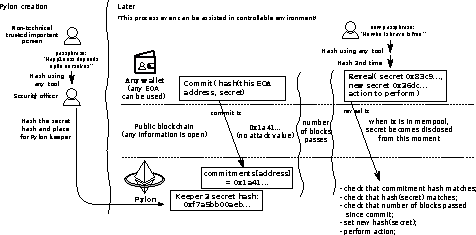
\includegraphics[width=1.35\textwidth]{pylon_identity_protection.pdf}
    \caption[Figure 1]{Scheme for identity protection signing with arbitrary data\label{fig:identity_protection}}
%  \end{center}
\end{figure}



\bigskip

\subsubsection{Access control transparency}


To sum up, the ways to provide signing of a pylon state-change, the following methods can be used:
\begin{enumerate}
\item{A direct call from the EOA (or a smart contract, for example, a multisig) that is set for a keeper. Transparent and as secure as ETH;}
\item{A call from any EOA using a signed message. Useful for producing an offline signature, and signing from another device. Signer address can be recovered from the message and signature. Signer address can be a 'fresh' generated ETH address;}
\item{A call using a single-time byte sequence producing a matching hash (and providing a new one). Signer identity is concealed and can be executed from third-party EOAs. \emph{Access can be transferred without the blockchain interaction};}
\end{enumerate}

For the pylon auditors, active methods for every keeper are fully disclosed as pylon contract view methods if both an address and single-time hash access are set. The keeper can change access parameters for itself using the same authentication method as approving pylon state change. Any actions produce corresponding events to allow for easier audit.

\bigskip
\subsection{Time-related and action-related constraints}
\label{constraints}

\subsubsection{Time-constrainted activation}

When permission to execute some activity is granted, it could (and for better security, should) contain time constraints. In case of permanently- given permissions, they should be reviewed and deactivated when required. Old addresses should not be exposed, or if permissions are still present could lead to an exploit. Or, as time goes, the situation could change, actors could behave differently.


The ability to set time constraints is one of the most critical and distinctive features of pylons. When performing a pylon activation, the state change could specifically have time constraints set:
\begin{itemize}
\item{a duration set in seconds;}
\item{an active state end timestamp;}
\item{an active state end block.}
\end{itemize}


Pylon can be deactivated (with sufficient power) at any time, but time-constrained activation reduces the amount of aftercare and the risks related to security maintenance.

Pylon can be queried for the remaining time or number of blocks it would stay in an active state.


\subsubsection{Action-constrainted activation}

Pylon is the bearer of privileged actions. Meaning the particular pylon address is has roles, ownership, or another form of privileged execution set in target contracts. However, it is possible to add additional restrictions or narrow down possible execution actions, allowing for several possible constraint levels:
\begin{itemize}

\item{No constraints. Pylon is acting as an \emph{execution proxy}. Providing the ability for the pylon executors to call any method in any contract address (this would also allow pylon to act, for example, like shared storage of ERC20 tokens). It’s possible to call ERC20 transfer methods, for example, but only for trusted executors;}
\item{Contract address constraints. Executors can call methods through pylons only for allowed contract addresses;}
\item{Method-level constraints. Executors can only call methods for a contract with matching signature (following the traditional EVM method signature as restriction format);}
\item{Parameter-level restriction. Executors can only call specific methods for which a parameter restriction could be set. For example, 1st parameter for method 0xa1b2c3f4 should equal true (0x0000...0001). EVM external types uint256 notation specified.}
\end{itemize}

This action-constraint granularity allows attaching pylons in scenarios where the target contract is not supporting roles. Where roles have exhaustive permissions or methods that cannot be fully allowed. For example, attaching pylon as the owner of a contract, but restricting the available actions for the executor, while not allowing to further change owner. This constraint could be lifted later if such a need arises through constraint change and reactivation by pylon keepers.


\subsubsection{Permission quantification}
\label{permission_quantification}

For certain sets of actions, there could be a requirement to limit the interaction level measured in some numerical value. Possible examples that require the use of this feature:
Possible examples that require use of this feature:
\begin{itemize}
\item{An investment strategy that has only a certain amount of funds allocated to it;}
\item{An ability to make payout transactions from a contract, but with a maximum value cap to protect funds;}
\end{itemize}

Call-level constraint: at the \emph{end of interaction execution}, pylon checks if a value returned by a defined call data is less than a predefined value, for example, fundsAllocated(address) is less than 120,000).

Single-parameter thresholds can be set to limit the maximum parameter value in a particular method. Two additional constraints can be specified for more practicality:
\begin{itemize}
\item{A timeout in seconds after method execution call (so that a large value cannot be produced by spamming small transactions) also helps with recurrency attacks;}
\item{A cumulative parameter threshold for all method calls, when every single parameter value in different calls is capped. And the total value is checked against the threshold;}
\end{itemize}

Call-level check is defined for the whole activation state, while tuple of parameter maximum constraint, total collective amount, and timeout are specified for one or more function signatures.

Note: when pylon activation parameters ('charge') are limited for some functions, there is no distinct accounting for different executors. It is implied that when keepers charge pylon, they evaluate the overall maximum quota for some objects. In case it should be different, different pylons should be used.


\subsection{Keeper power and vetoing}


Pylon keepers have power (can be called voting power) set within a particular Pylon.
Every Pylon has $P_A$ activate power threshold set and can also have a veto $P_V$ power threshold set (if $P_V$ is not set, it equals to activate power threshold $P_A$).

\medskip
Activate power threshold $P_A$ is a value, which must be reached by a keeper (or a group of keepers) for:
\begin{itemize}
\item{Changing the Pylon state to active, alter active state parameters, or changing state to inactive;}
\item{Modify Executors for a Pylon;}
\item{Modify Keepers for a Pylon, (if Pylon is not in the state of lockdown);}
\item{Propagate a new pending state another Pylon, for which this one acts as a keeper;}
\item{Approve a pending state for another Pylon, for which this one acts as a keeper;}
\end{itemize}

\medskip
Veto power $P_V$ is a value, which must be reached by a keeper (or a group of Keepers) for:
\begin{itemize}
\item{Power down the Pylon (e.g. when this could be needed quickly);}
\item{Put the Pylon in locked down state, effectively preventing even parties having $P_A$ voting power to change state or Keeper/Executors (for emergencies);}
\end{itemize}

Balancing the values of $P_A$ and $P_V$ allow more fine-grained control over the security. Especially for cases of a smaller number of actors. Besides, pylons are primarily designed to have a single-digit number of actors. So the blocking right could (or could not) be required, depending on the structure and the type of execution a particular pylon is providing.

\subsubsection{Two-keeper case and lockdown}


When pylon only has two keepers, there are several cases, when it is impossible to verify what actor or party should be blocked using any data available on-chain. It is also impossible to grant another actor or party the ability to recover access and security. For example, when both signatures are required from both keepers. Another example is when a single signature is required from any keeper (so they have equal rights). Finally, in situations when the keeper has enough power to modify the pylon state by its discretion, for example, if an actor decides to act maliciously (or another party acts maliciously).

This is somewhat similar to the ”two-generals problem”, or even more closely, relates to the fact that Byzantine Generals Problem (BGP) has no solution in this case. For example, three generals and one of them being a traitor. A simple explanation is that a loyal general can not determine which conflicting information to trust between the other loyal general and the traitor.

\smallskip
In such case, the only options that remain are:
\begin{itemize}
\item{Lockdown the pylon and halt its activity. Can be initiated by keeper or a party, cumulatively having power greater or equal to a veto threshold. This operation cannot be canceled by other keepers when pending. Only when the initiator removes this lockdown. However, having enough power for a veto threshold won’t allow such party to change pylon state or alter keepers set;}
\item{If pylon has an emergency committee set (which can be represented as another pylon, EOA having special security level, DAO contract, etc.). Only such actors can alter pylon keeper set and provide means to recover and unlock the pylon.}
\end{itemize}



\subsubsection{Pylon state}

To avoid complexity overhead and considering additional risks, pylons have a maximum of two state definitions that are stored in the contract:
\begin{itemize}

\item{Active state definition. \textbf{Offline} or \textbf{active} (inactive state can be an additional action and time constraints set). In case of emergencies, pylon can also be in a \textbf{lockdown} state. In this case, it cannot change state until resolved by Emergency committee (\ref{emergency_committee});}
\item{Pending state definition. This state change can be proposed by any keeper. Other keepers can approve (if required) resetting of the previous pending state. After reaching the activation threshold $P_A$ it immediately becomes an active state.}
\end{itemize}

Pylon state definition contains activation time and action constraints (what contracts/methods can be called along with parameter restrictions and call timing restrictions). To concisely compare if the pylon state is the same, a \textbf{fingerprint} of the definition is done, being essentially the hash of the state definition data.

For a full description of what is included in pylon state, check the \ref{state_reference}.

\subsection{Keeper and Executor management}

As any keeper can propose a new pending activation state, a malicious keeper could disrupt the pylon operation. For pylon administration, pending administrative action is recorded by each keeper separately.

For example, in $Pylon(2, 1, 1, 1)$ (three keepers with power 1 each, $P_A = 2$), if keeper A proposes administrative action to 'remove keeper C' at any time. Keeper B could sign this, and keeper C cannot interfere with such action even if they propose another action, for example, 'remove Keeper C'.

The administrative actions are following:
\begin{itemize}
\item{Add a keeper, providing voting power and address or single-time hash;}
\item{Change keeper voting power;}
\item{Remove keeper;}
\item{Add executor, providing address;}
\item{Remove executor.}
\end{itemize}

The ability to self-administer keepers and executors within the pylon provides managed mutability to the security infrastructure. It allows for a gradual introduction of new actors or expansion of hierarchy when deemed necessary.

Keeper can be one of the following:
\begin{itemize}
\item{Externally-owned address ('regular' wallet, or hardware-protected, etc.);}
\item{Another pylon (usually without executors, so called 'Actor Pylon');}
\item{Smart contract;}
\end{itemize}

When pylon acts as a Keeper it has one major difference from other types of Keepers. When the state fingerprint of the pylon remains the same, the keeper pylon provides 'power' to the kept pylon if it is active itself, or stops providing power when it goes offline (or when the state fingerprint of pylon being kept changes). This allows building convenient patterns for maintaining security infrastructure.

In addition, pylon has two methods to act as a keeper for another pylon: a method to propagate/propose state change for another pylon or approve proposed state change. In the case of arbitrary smart contracts, these methods can be implemented, but will require additional effort and probably should be left out for non-standard scenarios.

\subsubsection{Pylon types}

The division is completely artificial (the Pylon contract implementation logic and code should remain the same), but some distinct types can be put into classification.

If pylon provides execution, it can be referenced as ``Execution Pylon''. If pylon has keepers set, but no executors, it can serve as a unit of security for other execution pylons (some situations are illustrated in section \ref{situation_modelling}, ``Situation modelling'').

A pylon can be called ``Actor Pylon'' when it represents an single entity (a person, company, unit, etc.) and does not provide execution (has no Executors defined), only serves as Keeper for other pylons.

For other special case, pylon can be called a ``Multi-Sig Pylon''. When all executors are also keepers. And the usage pattern is when pylon is activated -- action constraints specify a single method call with defined parameters (the other keepers must approve). The action limit for a state is set to 1 on every activation. In such a scenario, pylon would act almost exactly as traditional on-chain multi-signature wallets (allowing to perform single action when activation threshold is reached).

\subsection{Actor Pylons and composability}
\label{actor_composability}

The ability for pylon to be a keeper for another pylon is critical. When pylon, which address is set as keeper is in the active state, it \emph{could be} automatically assumed by the dependent pylon that any state change or administrative actions are supported by its' keeper voting power.

This property is important, it is specified upon pylon construction and called ``passive approval''. If it is set to true, when the Pylon is active, it \emph{automatically provides his voting power to wherever it is set as Keeper}.

Such a feature allows:
\begin{itemize}
\item{To have an entity present which could maintain the state of its Actor pylon, minimizing the overhead of diving into particular execution pylons, but having the ability to stop any action instantly by deactivating its' pylon;}
\item{To reduce security management overhead (frequency of actions needed for reactivation, etc.), that could impact effectiveness, esp. in rapidly changing conditions;}
\end{itemize}

With great power comes great responsibility. The security should be properly structured (which is always the case anyway).

\subsection{Emergency committee}
\label{emergency_committee}

This is a single address (that could be EOA, multisig, or, more practically, another pylon) with the ability to perform unique security-elevated actions. Emphasis on the term 'committee' is to reflect that best practice would be not to make a single EOA act in this role. An emergency committee may not be set in the pylon at all, and in such a case, this could not be changed.

Emergency-related actions are following:
\begin{itemize}
\item{Replace emergency committee address to another one (removing current committee address);}
\item{When pylon is in lockdown state, remove any keeper or executor (note: emergency committee does not allow changing or adding keepers or executors if the control over pylon is lost that remaining trusted keepers do not have enough power to manage it, then it’s practical to leave it locked down and create a new one, and in addition reassess the security situation);}
\item{Unlock pylon that is in lockdown state (and only the emergency committee can do this);}
\end{itemize}

It is not by any means required to set the emergency committee address for the pylon, as the emergency committee has elevated power over the pylon, it is worth noting that these permissions \emph{cannot affect the pylon behavior until it's in lockdown state}. The goal of the emergency committee is to resolve critical conditions that could not be solved by the pylon keepers.

\subsection{DAO Interactions}

One of the possible use cases for pylons would be to serve as a limit call proxy on the number of smart contracts where DAO decisions could programmatically trigger actions. Without over-exposure to available method calls. DAO smart contract handling and enabling (even performing) calls that change how the governed contracts behave.

For example, a DAO can vote on collected protocol fees to be transferred to a specific wallet to incentivize new project development. Of course (this consideration is out of scope), such function could not be injected into a fee-distribution contract, but (just for example) it has methods to set the fee size and address to collect them too. Such constraints could be planned/defined through pylon and executed by any trusted party (or even anyone), but only if an on-chain condition on a DAO contract, proposal vote result, etc., matches the defined criteria.

\pagebreak
\section{Situation modelling}
\label{situation_modelling}

\subsection{Pylon notation}

A visual representation of a single pylon or pylon hierarchy can be useful for several reasons:
\begin{itemize}
\item{to concisely present the information, but in an easier to interpret way (for example, in comparison with table view), reducing the risk of human error;}
\item{to serve as a foundation for the UI of tools that can be developed for public disclosure, audit, or management of pylons infrastructure,}
\end{itemize}

\medskip


\begin{figure}[h]
  \hspace*{-1cm}
%  \begin{center}
%    \centering
    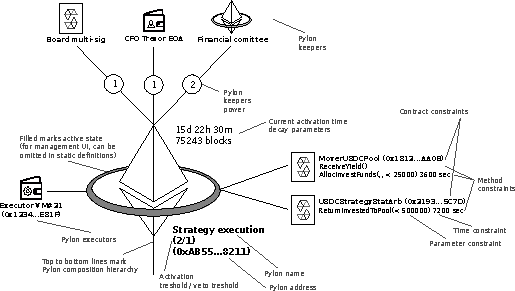
\includegraphics[width=1.25\textwidth]{pylon_sign_scheme_v2.pdf}
    \caption[Figure 1]{Pylon notation example\label{fig:pylon_notation_example}}
%  \end{center}
\end{figure}

\bigskip
The expanded view of a single pylon is presented on Figure \ref{fig:pylon_notation_example}.
From top to bottom, pylon composition hierarchy is connected (keepers and pylon interconnections), and, from the left to right, managed execution flow: executors and execution constraints.

\smallskip
On the provided example, the pylon is named ``Strategy Execution''. It requires the voting power of 2 to activate. The veto power set to 1. There are three keepers: a multi-signature wallet (represented by a smart contract); an externally-owned address marked as ``CFO Trezor EOA''; and another pylon (probably, Actor Pylon, not defined on the figure) named ``Financial Committee''.

\smallskip
The pylon is currently active. The current activation state will last for 15 days, 22 hours, and 30 minutes, or 75,243 blocks (whatever time constraint reached first).

There is one executor, marked as ``Executor VM\#21'' that can call three methods on two smart contracts. The first contract is called ``\texttt{MoverUSDCPool}'' with available methods ``\texttt{ReceiveYield()}'' (without any restrictions) and  ``\texttt{AllocInvestFunds}'' with the 3rd parameter of value less than 25,000 (only once in 3,600 seconds). The second contract is ``\texttt{USDCStrategyStatArb}'' with the method ``\texttt{ReturnInvestedToPool}'' where 1st parameter value must be less than 500,000 (only once in 7,200 seconds).

This is a trivial, and slightly theoretical example, but we can gather significant information on what power each executor has. How frequently pylon's activation must be refreshed, and what entities are acting as keepers. More than that, it is easy to observe that the ``Financial Committee'' pylon has the power to manage the state, but other keepers have veto power to deactivate (or even lock-down pylon) at their sole discretion.


\pagebreak
\subsection{Personal pylon}

This pylon pattern can be used by a single person (may not be related to their area of work or tasks involved). Let's imagine that a person (Alice) has a frequently used wallet. The same wallet address used from several devices (daily):
\begin{itemize}
\item{A desktop computer at home (e.g., Metamask wallet Chrome extension);}
\item{A laptop that is used at work, sometimes at home, at public places, road trips, where the address is used as Metamask wallet Chrome extension;}
\item{Mobile phone (carried constantly) that has a swipe-pattern lockset, where a Coinbase wallet is installed.}
\end{itemize}


\medskip
We won’t enumerate all possible negative events that may occur. However, to name a few: mobile phone lost, stolen, stolen on purpose to gain the address access, malware scraped private key from a device, same for laptop, forgotten remote access software, etc.

\medskip
If a single address is used for critical actions (it is detectable through the transaction history) this could pose a great risk of losing funds and control access to smart contracts.


\begin{figure}[h!]
  \hspace*{-1cm}
    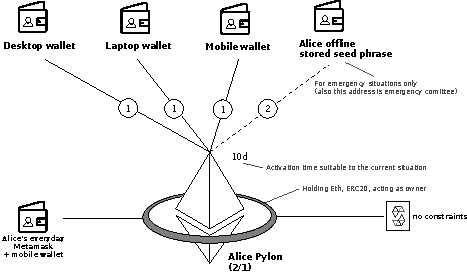
\includegraphics[width=1.15\textwidth]{pylon_example_personal_pylon.pdf}
    \caption[Figure 1]{Simple pylon pattern for personal use example\label{fig:pylon_personal_example}}
\end{figure}

Alice doesn't want the process to be overcomplicated. She doesn't have a hardware wallet or specialized devices, and she doesn't want to use a traditional multisig wallet. Sometimes she has a business trip or vacation and wants to interact with the blockchain without signing every transaction (e.g., she trades on a DEX, or has to make a payment). This process is cumbersome while using multiple devices.

\smallskip
\emph{Note that storing both multisig keys on one device is not the most secure way and ruins the purpose. Storing one key on a laptop and the other on a phone is less convenient. She won’t be able to execute if either the laptop or the phone is unavailable.}

\medskip
To separate responsibility and remove single point of failure an Actor pylon contract can be used by a person, consider the following example (Figure \ref{fig:pylon_personal_example}):

Pylon is created. Now, this contract serves as an address that stores assets (Ethereum, ERC20 tokens, etc.) and interacts with smart contract calls that require elevated permissions. Pylon is deployed with the following parameters:
\begin{enumerate}
\item{There is one Executor, the address that is frequently used and available across all devices;}
\item{There are no action constraints planned, meaning any contract, ERC20 interaction, or ETH transactions may be executed;}
\item{The activation power is 2, and the veto power is 1 (described in the next paragraph).}
\end{enumerate}

First of all, Alice generates a new seed phrase, takes the address, and sets it up as ``Emergency Committee'' and keeper with a power of 2. She breaks down the seed phrase on paper in halves and stores them in two separate secure spots. The procedure for emergencies: in case she loses control of the pylon, a malicious entity steals her device, unlocks it, and locks down the pylon (hopefully, this procedure will never be required).

Next, she decides to generate three different addresses (not derived from the same seed phrase!) on her devices: a desktop PC, a laptop, and a phone. All those three addresses are set as keepers for pylon with a voting power of 1.

When it has been all set up, the revised activity flow for Alice is as following:
\begin{itemize}
\item{During the regular daily routine, Alice reactivates pylon every two weeks with an activation time of 20 days. She can do that using any two of her three devices;}
\item{When her desktop PC is not available, she still has the voting power to control the pylon using a mobile phone and a laptop. For convenience, pylon can be activated for 30 days because of a business trip;}
\item{Pylon may be deactivated from any device instantly (because the veto power of 1 is set for it);}
\item{Alice could use the pylon for executing a transaction from any device without the requirement of producing multiple signatures, significant gas overhead, and other inconveniences.}
\end{itemize}


\emph{Note: This paper does not cover the UI for executing actions through pylon. A simple web interface that connects to web3 would be useful. It presents the ability to relay execution through pylons, e.g., a similar approach to different utilities with the MyEtherWallet service.}

\pagebreak
\subsection{Multi-keeper proxy pylon}

A simple example that still has practical value. It also is worth noting that simple solutions are often most effective and secure.

The purpose of this pattern is to provide execution to a trusted EOA (in possession of a person or an automated service), reducing the risk, but without the overhead of constantly being involved in signing every single action.

\begin{figure}[h!]
  \begin{center}
    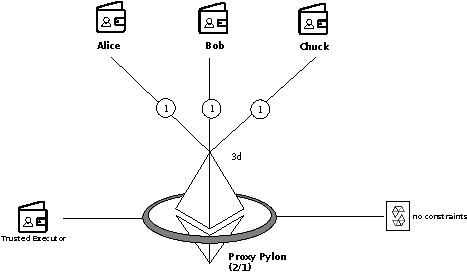
\includegraphics[width=0.95\textwidth]{pylon_example_proxy_pylon.pdf}
    \caption[Figure 1]{Pylon pattern for several keepers
    \label{fig:pylon_example_proxy_pylon}}
  \end{center}
\end{figure}

In Figure \ref{fig:pylon_example_proxy_pylon} a transparent proxy pylon is shown. Pylon is created with the following parameters:
\begin{itemize}
\item{Activation power of 2 (so any two of three keepers defined could activate it), the veto power of 1 so that every keeper can instantly shut down the pylon;}
\item{Activation is made for periods of 3 days and reactivated when required. No contract or method constraints are planned at the moment;}
\end{itemize}



\medskip
The benefits of using such a pattern are:
\begin{itemize}
\item{An ability to collectively govern the activities, while retaining the ability for every keeper to block the execution at any time;}
\item{The flexibility of changing the Executor (and Executor can be a completely separate entity, even a smart contract);}
\item{An ability to recover the state in case keeper loses the key (if keeper becomes malicious, it could lock down the pylon. However, the same addresses could form an "Emergency Committee" (e.g., in a generic multisig);}
\item{Depending on the level of trust, amount of controlled funds, or other changes, keepers can propose a different activation state, with stricter or more relaxed constraints, depending on the situation.}
\end{itemize}

For example, if Chuck loses access to his EOA (wallet), he could contact other keepers (Alice or Bob). Explain the situation, and provide a new address. They would have enough voting power to remove lost EOA and include a new one to recover from the incident.

Or, in case ``\texttt{Trusted Executor}'' could be compromised, to mitigate the removal of the old Executor and adding a new one should be required.

\pagebreak
\subsection{Pylon governed by a DAO}

Pylon has the ability to provide execution, only when a value of the call to another smart contract’s view function (described in \ref{permission_quantification} as "call-level constraint") allows creating pylons. Pylons that would be able to execute only when a specific on-chain condition is met.

\begin{figure}[h!]
  \begin{center}
    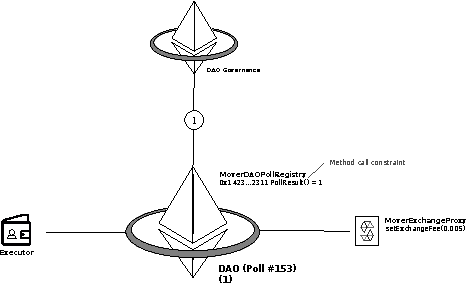
\includegraphics[width=0.85\textwidth]{pylon_example_dao.pdf}
    \caption[Figure 1]{Pylon pattern for a DAO voting result execution
    \label{fig:pylon_example_dao}}
  \end{center}
\end{figure}

Let’s consider a hypothetical situation (Figure \ref{fig:pylon_example_dao}). A poll is executed if the exchange fee could be set to 0.5\%. Thankfully, the result of a poll would be reflected in the contract "\texttt{MoverDAOPollRegistry}". Because of that, we can create a pylon, with call-level restriction checking for a specific value in other contract’s view function or a public variable. The action constraint also specifies the exact value matching the poll outcome that should be executed if the options win. In such a case, ``\texttt{Executor}'' can be any EOA, or a smart contract, because of the restrictions defined (if conditions are not met, the call will revert).

In addition, to mark that DAO is active, a DAO ``Governance Pylon'', potentially with many keepers acting as the board (the structure is not in the scope of the example) is set as a keeper for the ``\texttt{DAO (Poll \#153)}'' pylon. It provides an ability to block the execution. If that is not desired, a passive ``Actor Pylon'' is defined to be in the inactive unchangeable state forever.


\pagebreak
\subsection{Hiearchical placement}
One of the major features is the ability to place pylons in the hierarchy. It means that a pylon, as was already mentioned in \ref{actor_composability} could be a keeper for another pylon. In addition, such pylon can have a ``\texttt{passive\_approval}'' flag set. In such a case, pylon would automatically provide its voting power (if it is in an active state itself).

\smallskip

In the example in Figure \ref{fig:pylon_example_composition}, there is the ``\texttt{NFT Management}'' pylon. Its purpose is to grant minting ability to the Executor. Let’s imagine there are several people responsible for that particular NFT for the project. They are not technical and do not interact with smart contracts directly, yet, they monitor and maintain the actual activities related to NFTs. In this case, a passive ``Actor Pylon'' is constructed to represent their governance. It is active under normal circumstances. This approach relaxes management overhead for them. Only if they decide that something is wrong, they deactivate their ``Actor Pylon'' (``\texttt{NFT Management}''). When the situation resolves, the ``NFT Management'' team reactivates their ``Actor Pylon'' back to an active state. No other actions would be necessary from their side, providing a degree of control with minimal maintenance overhead.

\begin{figure}[h!]
  \begin{center}
    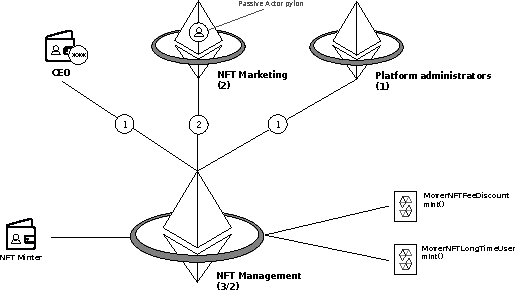
\includegraphics[width=1.00\textwidth]{pylon_example_composition.pdf}
    \caption[Figure 1]{Pylon composition with passive ``Actor Pylon'' example
    \label{fig:pylon_example_composition}}
  \end{center}
\end{figure}

There can also be hierarchy and composition from the Executor side (Figure \ref{fig:pylon_executor_composition}). The same Executor may be defined in several pylons, depending on the actions it needs to perform. It provides an ability to keep infrastructure compact, while not creating exceedingly many executors, pylons, and other entities. Bloated security infrastructure could eventually become less secure, because of complexity and maintenance requirements.

\begin{figure}[h!]
  \begin{center}
    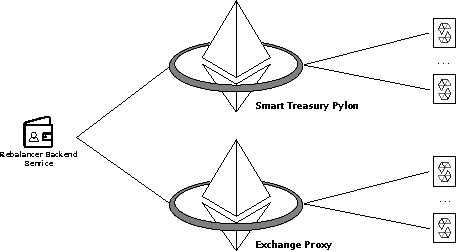
\includegraphics[width=0.95\textwidth]{pylon_executor_composition.pdf}
    \caption[Figure 1]{Executor composition across multiple pylons
    \label{fig:pylon_executor_composition}}
  \end{center}
\end{figure}


\pagebreak
\subsection{Risks and attack vectors}

Because of the flexibility, risk analysis is required when deploying and using complex smart contract structures. It includes pylons as well.
This is an incomplete checklist, but the following assessions should be made:
\begin{itemize}
\item{Is the composition of keepers and their voting power balanced? (Especially if a single keeper has voting power that is sufficient for activation, same for the veto power);}
\item{Do all keepers ensure a proper key storage security?}
\item{What are the procedures and "Emergency Committee" if the pylon gets in the lockdown state?}
\item{Are time and action constraints strict enough to ensure the safety margin of the underlying execution flow?}
\item{Is pylon detached, or is it upgradeable (or part of upgradeable infrastructure)? Who has the ``\texttt{UPGRADEPROXY\_ADMIN}'' role, and is it secure enough?}
\end{itemize}

Some (pylon-specific) attack vectors may include:
\begin{itemize}
\item{Upgrading pylon contract (if it is upgradeable);}
\item{Denying (shutting down or locking down pylon) execution if a malicious actor gets voting power equal to the veto power;}
\item{Possessing the control over the pylon in case a malicious actor gets voting power equal to activation power;}
\item{Possessing control over the Executor (Especially if action constraints are too relaxed).}
\end{itemize}

Security is very frequently a balance of convenience and safety. The correct arrangement and configuration of pylons would require an understanding of how they work and the main principles (although the workflow for keepers is kept simple).

\pagebreak
\subsection{Use cases for a DeFi service infrastructure}

For the next several examples, let’s consider the following roles in the project (company), working in Decentralized Finance (DeFi), building and operating a product/service related to non-custodial fund-like management of user assets. Each role corresponds to a separate person or team:
\begin{itemize}
\item{CEO, responsible for the overall operation;}
\item{CTO, responsible for technical architecture and development;}
\item{CFO, responsible for accounting overview, activity audit, and analysis of financial results;}
\item{Security Officer, responsible for security audit, maintenance, and related activity analysis;}
\item{The savings team develops and maintains the Savings product feature (similar to deposits/investment activity);}
\item{Platform administrators take care of smart contracts related operations executed manually (most administrators are also project developers);}
\item{Backend EOAs, wallets controlled by automated backend services to perform automated execution of various methods of a project's smart contracts;}
\end{itemize}
As the project aims to keep a compact structure, the CFO is also acting as a Treasurer. This role is to be governed by the DAO in the future.

Every person was instructed about the keys storage procedure (encrypted with a password). The Security Officer holds one of the keys in an offline location and signs messages offline. They provide signatures off-chain from another wallet (which is changed from time to time at their discretion, as described in \ref{sec_interaction_flexibility}).

When CEO and CTO wallets are presented in the figures they have an additional complicated secret phrase set up, marked by “***” badge (this could be a key). The actual data is not disclosed to anyone and not stored on any electronic device, as described in \ref{sec_identity_protection}.

\pagebreak
\subsubsection{Financial strategy Pylon}
\label{example_fin_strategy_pylon}

\begin{figure}[h]
  \hspace*{-1cm}
%  \begin{center}
%    \centering
    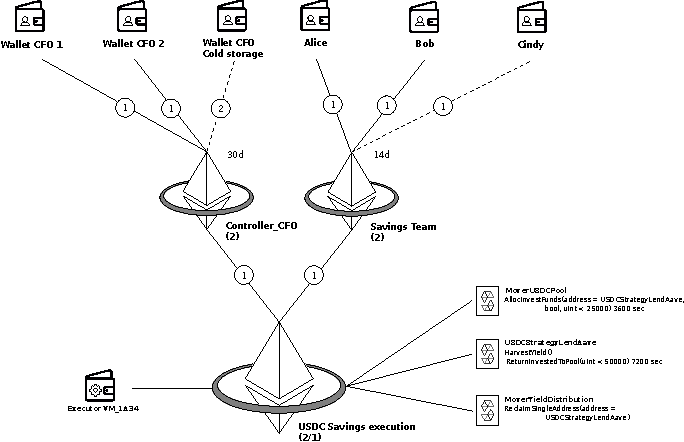
\includegraphics[width=1.25\textwidth]{pylon_example_strategy_management.pdf}
    \caption[Figure 1]{Example use case: Financial strategy management Pylon\label{fig:pylon_example_strategy_mgmt}}
%  \end{center}
\end{figure}
%pylon_example_strategy_management.svg

In the following example (Figure \ref{fig:pylon_example_strategy_mgmt}), let’s consider the process of managing funds for a financial strategy (USDCStrategyLendAave). This strategy is executed from an EOA (Executor\_VM\_1A34) owned (including the private key) by an off-chain backend service. The service performs actions at its discretion, for example, harvests yield when gas price is sufficiently low, and the available claimable amount is above a certain threshold.

This process is permitted by the two groups represented by two Action Pylons. The first (Controller\_CFO) is a dedicated pylon that is managed by the company’s CFO (Chief Financial Officer). It is activated for a longer period (of 30 days) using two private keys stored separately. Activation requires signatures from both keys at a convenient schedule at the end of every 4th week. The CFO has calendar events scheduled to keep pylon activated, which is done from two separate devices during the day, where the keys are stored. However, there is also a third EOA (Wallet CFO Cold Storage) with sufficient voting power to block the pylon or manage keepers, if one of the keys is stolen, or even both other keys are lost. If both keys are stolen by a malicious third party, he would still be able to put the pylon in a lockdown state. When performing reactivation, the CFO can overview the performance and results of the managed process.

The strategy is mainly engineered and maintained by a team of three people: Alice, Bob, and Cindy. Each actor has their EOA as keeper in the Savings Team Actor Pylon, which represents them as a single responsible entity for the process. Currently, Cindy is on vacation and does not perform any activities. Alice and Bob review the results of strategy performance every Friday and reactivate the pylon for the next 14 days. To have some additional time if someone doesn’t manage to put their signature on time.

When both CFO and Savings Team Actor Pylons are active, they act as only two keepers for the USDC Savings Execution Pylon. It allows the EOA Executor Executor\_VM\_1A34 (a host in a cloud provider tagged 1A34 for matching convenience) to trigger transaction method calls in the following smart contracts: MoverUSDCPool, only method AllocInvestFunds, with 1st parameter address equal USDCStrategyLendAave address and 3rd parameter that should be less than 25,000 e6, and with the time constraint of doing that only once per 3,600 seconds; USDCStrategyLendAave, two methods, HarvestYield() without any constraints and ReturnInvestedToPool, with first parameter less than 50,000 e6 once per 7,200 seconds; MoverYieldDistribution contract, ReclaimSingleAddress() method where 1st parameter is the address of the strategy USDCStrategyLendAave, without time constraints;

This example highlights the following features:
\begin{itemize}
\item{Responsibility separation. CFO and Savings Team under normal circumstances, only manage their Actor Pylon and on their schedule, matching their level of involvement;}
\item{Limitations of what automated executor can do (yes, the underlying software logic should be aware of at least not conflicting with action and time constraints that are defined), limiting the risk, including quantitative restrictions;}
\item{These restrictions are managed by the Savings Team. If they need to change them, they propose a new pending activation state. It should be approved by the CFO (during this process pylons stay active and the process does not get interrupted).

As was described in \ref{actor_composability}, Pylon has a special method to propagate state change to the pylon for which it acts as a keeper (or approves such change). It is like regular EOA keepers do, but with one key difference: if the actor pylon becomes inactive, it would automatically mean that its voting power does not count towards the pylon it is keeping. And vice versa, if the pylon becomes active, its voting power is returned, but only if the activation state fingerprint of the kept pylon does not change (this means primarily that action constraints and time constraints do not change). Regarding the example, USDC Savings Execution pylon activation has no activation time decay. Even if one of the keeper pylons goes down (for any reason) and then becomes active back, the USDC Savings Execution Pylon would resume its active state. However, to propagate the changes to the constraints, the Savings team should receive explicit approval from Controller\_CFO pylon (an action that requires the same voting power as its activation, in our case, signatures from both CFO EOAs).}
\end{itemize}

\pagebreak
\subsubsection{Asset Pool Pylon}

\begin{figure}[h!]
  \hspace*{-1cm}
%  \begin{center}
%    \centering
    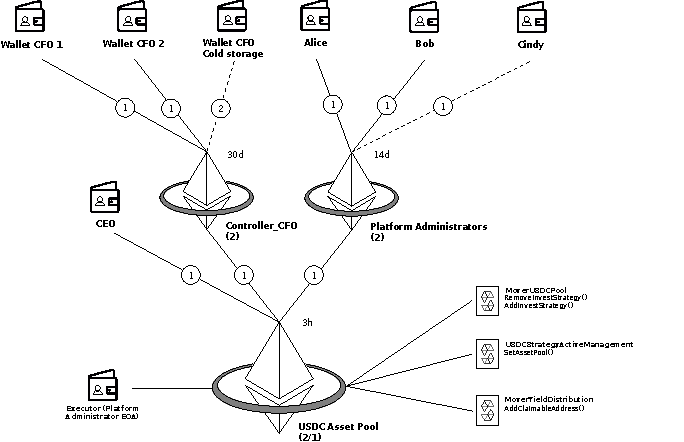
\includegraphics[width=1.25\textwidth]{pylon_example_pool_management.pdf}
    \caption[Figure 1]{Example use case: Asset Pool management Pylon\label{fig:pylon_example_asset_pool_mgmt}}
%  \end{center}
\end{figure}


Now let's consider an example for managing the asset pool itself. We don't dive in (and in fact, may not even know the details of how a particular investment strategy performs execution).

Note: the CFO Pylon could be \emph{the same} for example, the same pylon used in the previous section \ref{example_fin_strategy_pylon}).

These actions are not frequent and not automated. The executor is an EOA that is operated by financial management (it does not need to be multisig, etc., as the pylon is \emph{activated on demand}. It e a window for a trusted executor to perform pool management actions (thus, it can be performed with corresponding control and monitoring).

The ``\texttt{USDC Asset Pool}'' is activated for a short period (e.g., three hours), and to provide additional security, could be deactivated at any time by one of the Keepers (e.g., when required management operations are successfully finished).

The assumed process is slightly different. Pylon stays offline most of the time, not exposing any custodial risk to the asset pool.

When it is required to make some changes to the pool, e.g., completely remove an investment strategy (we assume the method ``\texttt{RemoveInvestStrategy}'' also make a call from a pool to a strategy smart contract to return invested funds). In this scenario, after the decision was made and confirmed, the ``USDC Asset Pool'' pylon needs to be activated to perform this maintenance.

At any time, CEO can stop the execution using his EOA directly, such ability has CFO through his ``\texttt{Controller\_CFO}'' pylon and platform administrators through their pylon.

Actions that could be performed through method level constraints are observable, so when the active state is proposed by platform administrators, CFO and CEO can review it and approve if they agree with the actions allowed to be made, within time window of 3 hours.

After the Pylon activates, Executor performs the actions, upon success, Platform Administrators shut down the pylon (as their voting power of 1 is equal to pylon veto power of 1).

The pylon helps to align the security with the process and all parties have a degree of security control matching their roles.

\pagebreak
\subsubsection{Infrastructure management Pylon}

\begin{figure}[h!]
  \hspace*{-1cm}
%  \begin{center}
%    \centering
    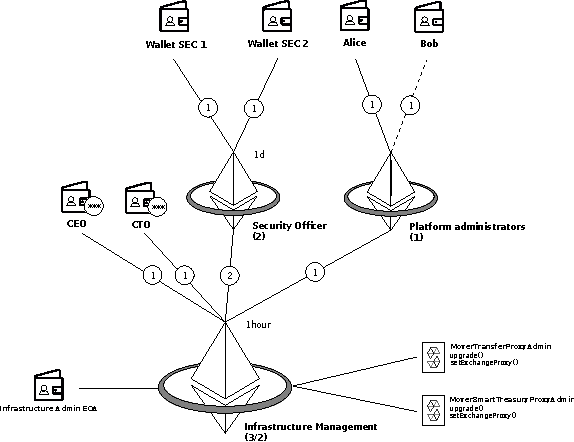
\includegraphics[width=1.25\textwidth]{pylon_example_infrastructure.pdf}
    \caption[Figure 1]{Example use case: Infrastructure management Pylon\label{fig:pylon_example_infrastructure}}
%  \end{center}
\end{figure}

Infrastructure Management Pylon(s) serve for access to a smart contract infrastructure maintenance (not related to other pylons), the primary purpose is to provide means for deployer role to upgrade smart contracts when required.


Pylon's address acts as \texttt{ADMIN\_UPGRADE\_PROXY} role for most of the project smart contracts that are upgradeable. The pylon has an activated power of 3 and veto power of 2, having the activation duration set to 1 hour. These values were chosen to align with the workflow and the following possibilities:

\begin{itemize}

\item{During the \emph{regular workflow}, when the upgrade is planned (and announced) and the time is chosen, any available platform administrator(s) propose(s) to activate the upgrade using their "Actor Pylon". They can also check that Executor EOA is set correctly and place appropriate action constraints. A Security Officer validates requested permissions (similar to performing a code review before merging the pull request) and approves activation through their "Actor Pylon". This results in achieving a voting power of 3, and the "Infrastructure Management Pylon" becomes active for a 1-hour time window to perform the upgrades;}
\item{In \emph{urgent} situations, upgrade activities can be performed by any of the following combinations: CEO and Security Officer; CTO and Security Officer; or CEO, CTO, and at least one Platform admin.}
\item{Security Officer can deactivate the pylon at any moment at their sole discretion. So can CEO and CTO, or CEO/CTO with at least one platform administrator. If there is a security breach or another serious means, the same consensus could be used to put ``Infrastructure Management Pylon'' into lockdown state until the ``Emergency Committee'' hopefully resolves the situation and provides means to recover access;}
\end{itemize}



\pagebreak
\subsubsection{Elevated actor Pylon}

``Actor Pylons'' serve to represent people or organizational units that prolong the validity of security and remove the single point of failure through the usage of multiple keys (or other means of providing actions). The main idea is to have timed permissions set, which can be extended for a specific period (e.g., every month). An incentive to review that all execution (which such pylon grants) is going as expected.

There could be several actor pylons created (including non-technical project participants), for example, for Marketing or promotion teams, project partners (and others), so they could have a degree of control where applicable.

The other benefit is separation between inner maintenance of an ``Actor pylon'' (person taking care of his keys, passwords, etc.) and maintenance of the security infrastructure, thus, if Alice changes her keeper EOA in her ``Alice pylon'', no actions are required from security officer (if it is assumed that ``Alice pylon'' is representing her as an actor and it's her responsibility to maintain it).

\subsubsection{Emergency Pylon}

The ``Emergency Committee'' is, as stated in its name operates during emergencies. It implies that people that are keepers store their access through an EOA or secret separately. And it is not used in other activities.
They are also should be trusted enough to possess such power. There are two considerations worth noting again:
\begin{itemize}
\item{The emergency committee \emph{cannot affect in any way} a normally functioning pylon unless it was put into the lockdown state;}
\item{The emergency committee should understand their composition and that only trusted members acting in good faith are having voting power there. If byzantine trust is not reached in it. There are \emph{no other means} to resolve the situation for locked down pylons if the emergency committee itself has been compromised and cannot act.}
\end{itemize}


%\subsubsection{Fee management Pylon}
%\subsubsection{Treasury management Pylon}

\pagebreak
\noindent \textcolor{gray}{\small{following sections (4, 5) contents are to be updated as implementation progresses}}
\section{Implementation details}

\subsection{Main interfaces description}
\subsection{View functions}
\subsection{Creation options}





%User interface pylon spawning and management prototype (addresses weights privacy parameters dashboard for creation -- through web interface, like gnosis does for multisigs)

%Veto blocks pylon execution (keepers 'sum' negative power together)

%                               30
%                 |--------------              | executing power: 30
%--|--------------|
%         10
%veto power: 10 (activated)


%Committee model, quadratic model







%Shares generation on local software
%then construct pylons with secret shares


%To help with human-errors and network-levels errors (off-chain), etc.



%Difference between pylon and multisig:

%- Pylon is activated for a period (could be deactivated immediately),
%  is such case it acts as a proxy from a single wallet, without any
%  overhead of multiverification
%  (separate security to different wallets, with auto-expiration);S

%Different pylons are used for different management activities (roles);



%- Auto-decay;

%- Variable per-user charge time;


%- Reconfigurable mesh;

%- Resilient to single-point failures;







%- Shard responsibility;
%- Remove single point of failure;
%- Provide ability to recover;
%- Manage roles across different contracts uniformly;
%- Time decay (don't leave forgotten open doors);
%- Ability to create separate key pair (not requiring eth/gas) and interact from any address not compromising security;



%Pylons of several types (division is artificial):
%1. Actor pylon (EOA belonging to person or service), named;
%	- actor can charge it's own pylon, then the meshed execution pylons update %their charge status;
%	- actor maintain list of trusted executor addresses;

%2. Execution pylon, having a number of executable actions set that can be %triggered by actor, semantically named;
%	- when charge status changes, pylon forms list of trusted executors;
%
%	- if execution actions are changed, pylon would require re-charging;

%Pylons form a mesh that grants or removes their power using a trust graph

%Simple case (like a 2/3 multisig):

%
%      /\\         /\\        /\\
%      \\/         \\/        \\/
%      user1      user1     user2
%      1/2        2/2       1/1
%
%        \\        |       /
%         \\       |      /
%          \\      |     /
%
%                 /\\
%                 \\/
%                 treasury mgmt
%                 2/3 actors required
%                 charge duration: 72 hours
%

%if a certain pylon gets compromised, then a call is made to linked pylons to %broadcast it's detach?


%Committee case: 3 actors, every actor has 2 signatures, 6 pylons in total
%execution pylon requires at least 2 signatures from 2 different actors

%if 1 actor is malicious -- it cannot make execution;
%if 1 actor fully lost it's signatures and 2 actors lost one of theirs system %is still manageable;

%actor can block its pylon (irreversible operation)
%actor pylon cannot block other pylon, only mark within itself in list of %blocked





%If Alice and Bob are peers, then in group of two it's impossible to arrange
%malicious actor protection. At least 2 of 3 actors is a minimal set.

%Actor pylon acts like a multisig, intended to be used by a single user,
%but user can add/modify any number of EOA signatures in it to his own %discretion.

%Actor pylon is charged/discharged by user with his signatures.
%Connected execution pylons are updating their status automatically.




%\subsection{Functional areas breakdown}

%The contract for Pylon contains several functional areas that should be separated and orthogonal \cite{wiki_orthogonal} to reduce security risks and possible side-effects of system behavior.

%\begin{itemize}
%\item Keeper-related functions (administration);
%\item Activation and state-related views;
%\item Keeper self-access modifying methods;
%\item Execution checks and execution methods;
%\item Pylon composition methods;
%\item Emergency functions;
%\item Pylon spawning, upgrading and detach;
%\end{itemize}


%\pagebreak
\section{Reference}


\subsection{Pylon architecture and interfaces}



\subsection{Pylon roles reference}


%\texttt{ROLE\_PYLONADMIN} Administrative role, handled by role manipulation functions

%\texttt{ROLE\_EMERGENCYCOMITTEE} Emergency recovery role, handled by role manipulation functions

%\texttt{ROLE\_UPGRADEPROXYADMIN}

%\texttt{KEEPER} Internal role in the Pylon contract logic

%\texttt{EXECUTOR} Internal role in the Pylon contract logic

%\bigskip


\subsection{Pylon parameter reference}

\subsubsection{Pylon global parameter reference}

%- activation power
%could be changed, action requires reaching previous value of activation power;

%- veto power
%could be changed, action requires reaching activation power.

\subsubsection{Pylon actor parameter reference}

\subsubsection{Pylon activation state parameter reference}
\label{state_reference}

%Change of any of the activation state parameters results in a change of activation state fingerprint, thus, discarding keeper approvals of previously pending activation.

%\smallskip
%time-based constraints:
%$\langle duration, deactivate\_timestamp, deactivate\_block \rangle$


%execution constraints:

%\smallskip
%for the execution call-level constraint:
%$\langle address, call\_data, maximum\_value \rangle$

%\smallskip
%for the method permission quantification:
%[
%$\langle cumulative\_threshold, maxvalue, timeout \rangle$
%]



\subsection{Implementation considerations}

\subsubsection{Possible management UI approach}

\subsubsection{Pylon spawning}

Pylons support the concept of 'spawning'. It means that a deployed pylon contract can spawn another pylon contract (holding the upgradeable proxy and the state), keeping the implementation \emph{the same as pylon through which spawning occurred}. This pattern provides the following benefits:
\begin{itemize}
\item{Uniformity of implementation and interfaces. It means pylon infrastructure can be maintained without additional toolings, like Solidity IDEs, etc. Note: when implementation is upgraded, it still should be upgraded for \emph{for all pylons that were spawned} to keep all pylons up-to-date;}
\item{Significant gas savings and lower maintenance requirements when multiple pylons use the same implementation contract, redirecting proxy to new implementation is orders of magnitude cheaper in gas costs;}
\end{itemize}

The ability to 'spawn' pylons is based on the transparent proxy pattern. It means it is enough to deploy a proxy contract with a custom initializer function to initialize the pylon state, but the implementation contract could be separate. The implementation is non-upgradeable. Only the pylon proxy (representing the pylon state) can be upgraded to point to a new implementation address.

Pylon can be deployed with the implementation contract that is already deployed on the Mainnet (as implementation at a particular address is immutable) not only from calls to other pylon but specifying the address of its implementation during deployment using \href{https://forum.openzeppelin.com/t/programmatically-deploying-upgradeable-proxies/4834/2}{ProxyFactory}\cite{ProxyFactory}.

As a step further, pylons can be deployed using not UpgradeableProxy pattern, but \href{https://docs.openzeppelin.com/contracts/3.x/api/proxy}{UpgradeableBeacon pattern ()}\cite{UpgradeableBeacon} that would allow to upgrade implementation for all spawned pylons in one transaction.

The upgrade role for the pylon infrastructure thus presents significant power and should be treated with sufficient security. If so desired, any pylon could be 'detached' making it non-upgradeable and fixed to current implementation logic.

\subsubsection{Pylon detach}

In case when increased security is desired, pylon upgrades proxy role can call the 'detach' method, which would set the upgrade proxy role to address 0x0000...0000, rendering pylon implementation immutable and non-upgradeable. This operation is non-reversible.


\pagebreak
\section{Definition of Terms}

\smallskip
\noindent \textbf{Activation} (pylon activation) -- a change of state of a pylon (from inactive/ shut-down state or another active state). Activation requires that keepers doing it have cumulative voting power equal or greater than the defined activation threshold $P_A$ (by proposing ``pending state'' and sequentially approving the change).

\smallskip
\noindent \textbf{Composition} (pylon composition) -- ability (and use pattern) of a pylon to act as a keeper for another pylon(s), forming pylon hierarchy and possibility to put one entity as executor for multiple pylons.

\smallskip
\noindent \textbf{Executor} (pylon executor) -- an internal role in a pylon logic, representing an entity (which could be: EOA or smart contract), that could perform actions through the pylon (by sending blockchain transactions) if the pylon is in active state, in accordance with the constraints defined.

\smallskip
\noindent \textbf{EOA} -- Externally Owned Address, a public-private key pair for interacting with Ethereum blockchain, where an Eth address is defined from a public key and private key could be used to sign valid transactions to be included in blocks.

\smallskip
\noindent \textbf{Keeper} (pylon keeper) -- an internal role in a pylon logic, representing an entity (which could be: EOA, another pylon, smart contract), which primary responsibility is to manage pylon state and activation state constraints. Each keeper has a voting power.

\smallskip
\noindent \textbf{Lockdown} (pylon lockdown) -- an state of a pylon, in which all functionality is put on halt, except calls from ``Emergency Committee'' (if it was defined for the pylon), primary purpose of the lockdown is to protect pylon in emergency situations (such as keeper acting maliciously).

\smallskip
\noindent \textbf{Pending state} (pylon pending state, pending activation state) -- a state of a pylon, that is proposed by (any) keeper of a pylon to replace current (active) state of a pylon. Other keepers can approve (vote towards the state change) or veto (vote against the state change). If cumulative voting power reaches $P_A$ activation threshold, pylon state changes to proposed one.

\smallskip
\noindent \textbf{State fingerprint} (pylon state fingerprint) -- a SHA3-Keccak hash of all pylon state parameters, including time constraints (time decay, timeout block, etc.), action constraints (allowed addresses, allowed method signatures, parameter constraints), call-level check and cumulative parameter threshold (described in \ref{constraints}).

\pagebreak
\bibliographystyle{abbrv}
\bibliography{simple}

\begin{thebibliography}{3}



\bibitem{bip47}
Justus Ranvier, BIP47
\\\texttt{\path{https://github.com/OpenBitcoinPrivacyProject/bips/blob/master/bip-0047.mediawiki}}



\bibitem{permissions_roles}
Open Zeppelin, Role-based permissions
\\\texttt{\path{https://docs.openzeppelin.com/contracts/2.x/access-control}}



\bibitem{OZ_SafeIERC20}
OpenZeppelin Github, openzeppelin-contracts  repository

\texttt{\path{https://github.com/OpenZeppelin/openzeppelin-contracts/blob/master/contracts/token/ERC20/utils/SafeERC20.sol}}



\bibitem{USDC_upgrade}
P.Kim, USDC v2: Upgrading a multi-billion dollar ERC-20 token

\texttt{https://blog.coinbase.com/usdc-v2-upgrading-a-multi-billion-
dollar-erc-20-token-b57cd9437096}



\bibitem{contract_forensics}
Smart Contract Research Forum, Blockchain is Watching You: Profiling and Deanonymizing Ethereum Users
\\\texttt{https://www.smartcontractresearch.org/t/ research-summary-blockchain-is-watching-you-profiling- and-deanonymizing-ethereum-users/564}

\bibitem{OnlineHashTool}
Online Tools, Keccak-256 Online encoder

\texttt{\path{https://webencrypt.org/onlinetoolsjs/keccak_256.html}}

\bibitem{FrontRunning}
Shayan Eskandari et al., SoK: Transparent Dishonesty:
Front-Running Attacks on Blockchain

\texttt{\path{https://users.encs.concordia.ca/~clark/papers/2019_wtsc_front.pdf}}


\bibitem{ProxyFactory}
Open Zeppelin, Upgradeable Proxies
\\\texttt{https://forum.openzeppelin.com/t/programmatically-deploying- upgradeable-proxies/4834/2}



\bibitem{UpgradeableBeacon}
Open Zeppelin, Upgradeable Proxy Patterns
\\\texttt{\path{https://docs.openzeppelin.com/contracts/3.x/api/proxy}}





\end{thebibliography}


\pagebreak
\tableofcontents



\includepdf{coverimg.pdf}

\end{document}
